\chapter{Introduzione}
\label{ch:intro}

\section{Il progetto SeismoCloud}

\begin{wrapfigure}{r}{0.25\textwidth}
\centering

\includegraphics[scale=0.15]{assets/01/logoseismocloud.png}
\caption{Logo di SeismoCloud.}
\label{fig:logo}
\end{wrapfigure}

SeismoCloud \cite{seismocloud}, il cui logo è mostrato nella figura \ref{fig:logo}, è un progetto rilevazione e segnalazione di terremoti basata su una rete di sismometri diffusi a livello nazionale. Il progetto nasce dalla collaborazione dell'Università degli Studi di Roma ``La Sapienza'' e l'Istituto Nazionale di Geofisica e Vulcanologia (INGV). Lo scopo del progetto è l'Earthquake Early Warning (EEW), che consiste nel controllo dell'attività sismica e, in caso di un terremoto, la notifica agli utenti interessati.

Poiché i sismometri previsti dal progetto sono a basso costo, sono imprecisi e pertanto solo con una grande quantità è possibile effettuare una stima affidabile del verificarsi di un terremoto. Per tale motivazione il sistema EEW non è attualmente abilitato. Ci sono più di un centinaio di sismometri attivi a livello nazionale, numero in crescita di anno in anno, ma, da come si evince dalla figura \ref{fig:distribuzione}, è necessario che siano ben distribuiti sul territorio.

Una funzionalità di SeismoCloud è la possibilità di formare dei gruppi di utenti, spesso organizzati dalle scuole, per condividere statistiche sui propri sismometri.
\begin{figure}[ht]
\centering
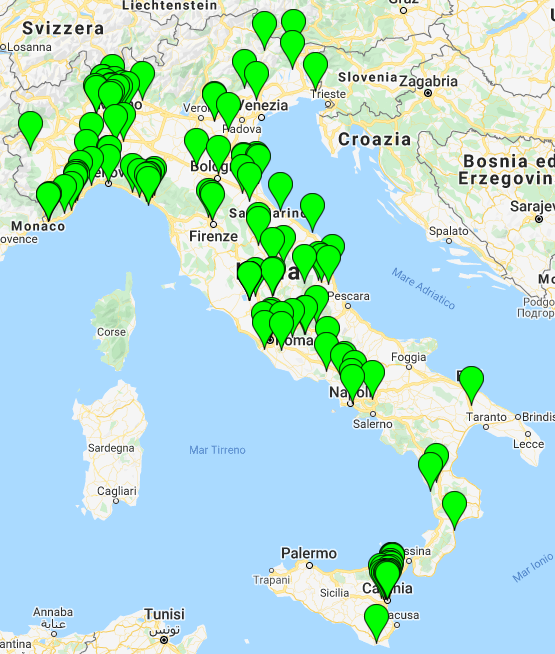
\includegraphics[scale=0.35]{assets/01/distribuzione_sismometri.png}
\caption{I sismometri attivi a livello nazionale.}
\label{fig:distribuzione}
\end{figure}

\paragraph{Tipologie di sismometri} I sismometri possono essere di due tipologie: una fissa costituita da dispositivi \textit{Internet of Things} (Arduino, NodeMCU e Raspberry PI) a basso costo e open source, che l'utente può costruire seguendo le istruzioni fornite sul sito web del progetto, oppure una mobile che consiste in un'applicazione per telefoni (Android e iOS).

L'applicazione mobile permette agli utenti di gestire e monitorare lo stato dei propri sismometri e della rete nazionale, in più rende il telefono esso stesso un sismometro, sfruttando l'accelerometro per rilevare le vibrazioni nei momenti in cui il telefono non viene utilizzato ed è poggiato su un supporto orizzontale.

Tutti i sismometri sono registrati all'interno del server di SeismoCloud. Ogni volta che uno di questi rileva una vibrazione, invia via Internet i dati al server, che tramite algoritmi dedicati, è in grado di capire se si tratta un terremoto nei primi secondi dall'inizio della scossa. Nella figura \ref{fig:rete} è possibile osservare il funzionamento della rete.

\begin{figure}[ht!]
\centering
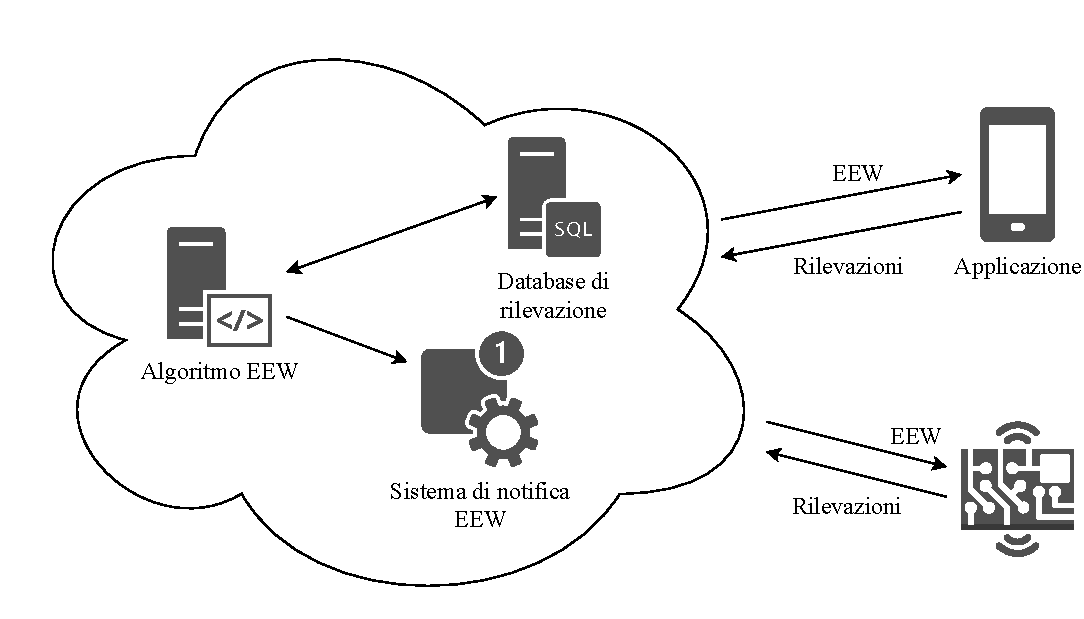
\includegraphics[width=\textwidth]{assets/01/rete.pdf}
\caption{Architettura della rete di SeismoCloud.}
\label{fig:rete}
\end{figure}

\section{Architettura server di SeismoCloud}

Prima di descrivere l'obiettivo del tirocinio, è utile tenere in mente l'architettura lato server di SeismoCloud, mostrata nella figura \ref{fig:architettura}. I vari client possono interagire con il server attraverso il protocollo HTTPS e MQTT su quattro componenti:

\begin{itemize}
\item \textbf{API firmware}: espone le API necessarie per aggiornare i sistemi dei sismometri fissi;
\item \textbf{Broker MQTT}: gestisce l'arrivo dei dati delle rilevazioni dei sismometri;
\item \textbf{API principali}: espone la maggior parte delle API di SeismoCloud;
\item \textbf{Keycloak}: espone il servizio di registrazione e autenticazione degli utenti.
\end{itemize}

Le API principali richiedono quasi tutte l'autenticazione, ciò viene garantito tramite l'utilizzo di \texttt{token} che il client invia in ogni richiesta e che il server può verificare. Keycloak eroga tali token ai client.

Nel sistema è presente MariaDB come database relazionale per la conservazione dei dati. Nello stesso database sono salvati sia le rilevazioni degli eventi sismici che tutti i dati relativi ai terremoti, ai gruppi, i sismometri e altro.

È presente anche un server di \textit{file storage} MinIO, in cui sono salvati i firmware da inviare ai sismometri fissi.

Il componente \textit{Worker} si occupa invece di lavori asincroni eseguiti in modo distaccato dall'interazione con i client, tra cui l'aggiornamento della lista dei terremoti nel database e l'invio delle notifiche ai client.

\begin{figure}[ht!]
\centering
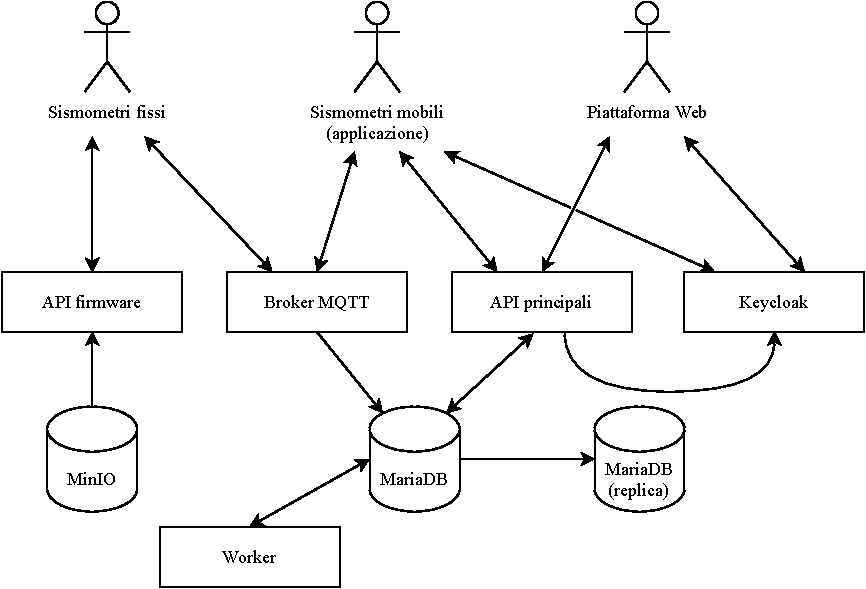
\includegraphics[width=\textwidth]{assets/01/architettura.pdf}
\caption{Architettura server di SeismoCloud.}
\label{fig:architettura}
\end{figure}

\section{Obiettivo del tirocinio}

L'obiettivo, svolto all'interno del team di sviluppo di SeismoCloud, consiste nella progettazione e nello sviluppo delle API per il servizio di messaggistica specifico per lo scambio di informazioni sui terremoti tra gli utenti. Tale funzionalità va a rafforzare lo scopo principale del progetto, cioè il servizio di EEW, in modo da aumentare, tramite l'interazione sociale, il bacino di utenti e quindi il numero di sismometri.

Il lavoro prosegue direttamente l'attività svolta dallo studente Michele Spina, che ha lavorato nello studio e progettazione dell'interfaccia utente per la funzionalità di messaggistica. Il suo lavoro è descritto in dettaglio nella relazione ``Design e development in Android dell’UI per l'interazione sociale in SeismoCloud'' \cite{michele}.